\documentclass[12pt, a4paper]{article}

\usepackage[
  margin=1in
]{geometry}

\usepackage[T1, T2A]{fontenc}
\usepackage[utf8]{inputenc}
\usepackage[russian]{babel}
\usepackage{minted}
\usepackage{tabularray}
\usepackage{siunitx}
\usepackage{graphicx}
\usepackage{multicol}

\graphicspath{ {img/} }

\begin{document}

\begin{titlepage}
  \centering
  \textsc{Новосибирский государственный технический университет}\par
  \vspace{1mm}
  Кафедра прикладной математики\par
  \vspace{4cm}
  \textsc{Практическая работа \textnumero 4}\par
  {\huge\bfseries Обходы графов\par}
  \vspace{1cm}
  {\scriptsize ФПМИ, ПМ-24\par}
  \vspace{1mm}
  {\itshape\large Параскун И., Шакиров П., Герасименко В.\par}
  \vfill
  {\small преподаватель\par}
  \vspace{1mm}
  \textsc{Домников Петр Александрович}
  \vfill
  \large{Новосибирск, 2024}
\end{titlepage}

\newpage
\setcounter{page}{2}

\section{Обход графа в ширину. Поиск кратчайшего пути}
\subsection{Постановка задачи}
\begin{itemize}
  \item Написать подпрограмму обхода графа в ширину из заданной вершины. На выходе файл с вершинами, перечисленными в порядке обхода.
  \item На основе подпрограммы обхода графа в ширину написать подпрограмму, выводящую кратчайший путь между двумя заданными вершинами.
\end{itemize}

\subsection{Текст программы}

\inputminted[firstline=9, lastline=27]{cpp}{/home/mehandes/c/src/github.com/meha4j/math/gmp/cpp/include/gmp_ucg.hpp}
\inputminted[firstline=11]{cpp}{/home/mehandes/c/src/github.com/meha4j/math/gmp/cpp/src/gmp_ucg.cc}

\newpage

\subsection{Результат выполнения}

\vspace{5mm}

\begin{multicols}{2}
\begin{minted}{console}
7   1 1 1 1 1 1 2 3 4 5 6 7
12  2 3 4 5 6 7 3 4 5 6 7 2

1: 2 3 4 5 6 7 
2: 1 3 7 
3: 1 2 4 
4: 1 3 5 
5: 1 4 6 
6: 1 5 7 
7: 1 2 6
\end{minted}

\columnbreak

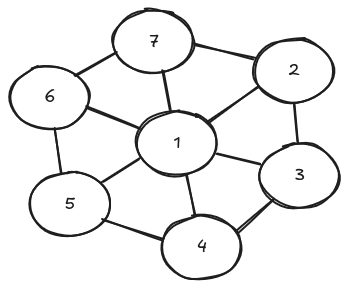
\includegraphics[scale=0.5]{1.png}
\end{multicols}

\begin{minted}{console}
[...]$ ./cmd/gmp/cpp/gmpcc-exe 1.txt 4 7
Shortest path: 4 1 7 (4 1 3 5 2 6 7)
\end{minted}

\vspace{5mm}

\begin{multicols}{2}
\begin{minted}{console}
7 1 1 1 2 3 4
6 5 6 7 3 4 2

1: 5 6 7
2: 3 4
3: 2 4
4: 2 3
5: 1
6: 1
7: 1
\end{minted}

\columnbreak

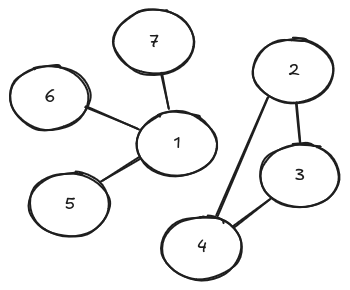
\includegraphics[scale=0.5]{2.png}
\end{multicols}

\begin{minted}{console}
[...]$ ./cmd/gmp/cpp/gmpcc-exe 2.txt 1 6
Shortest path: 1 6 (1 5 6 7)
\end{minted}

\vspace{5mm}

\begin{multicols}{2}
\begin{minted}{console}
7 1 2 3 4 5 6
6 2 3 4 5 6 1

1: 2 6
2: 1 3
3: 2 4
4: 3 5
5: 4 6
6: 1 5
7: 
\end{minted}

\columnbreak

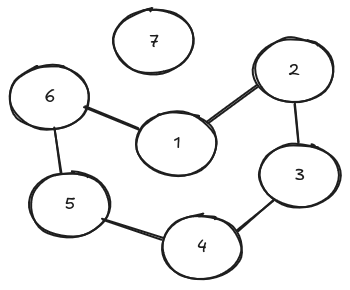
\includegraphics[scale=0.5]{3.png}
\end{multicols}

\begin{minted}{console}
[...]$ ./cmd/gmp/cpp/gmpcc-exe 3.txt 4 7
Path does not exists. (4 3 5 2 6 1)
\end{minted}

\vspace{5mm}

\begin{multicols}{2}
\begin{minted}{console}
7 1 5 6 2 3
5 5 6 1 7 4

1: 5 6
2: 7
3: 4
4: 3
5: 1 6
6: 1 5
7: 2
\end{minted}

\columnbreak

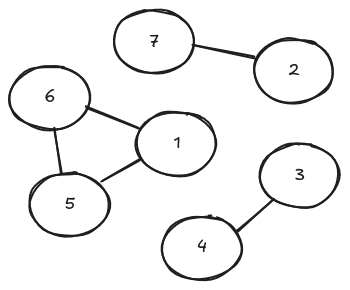
\includegraphics[scale=0.5]{4.png}
\end{multicols}

\begin{minted}{console}
[...]$ ./cmd/gmp/cpp/gmpcc-exe 4.txt 2 7
Shortest path: 2 7 (2 7)
\end{minted}

\vspace{5mm}

\begin{multicols}{2}
\begin{minted}{console}
7 1 3 2 7 6 5
6 6 2 7 6 5 4

1: 6
2: 3 7
3: 2
4: 5
5: 4 6
6: 1 5 7
7: 2 6
\end{minted}

\columnbreak

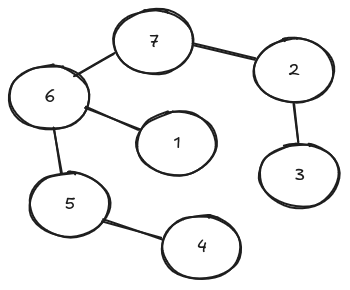
\includegraphics[scale=0.5]{5.png}
\end{multicols}

\begin{minted}{console}
[...]$ ./cmd/gmp/cpp/gmpcc-exe 5.txt 4 3
Shortest path: 4 5 6 7 2 3 (4 5 6 1 7 2 3)
\end{minted}

\newpage

\section{Объединение графов}
\subsection{Текст программы}

\inputminted[firstline=6]{cpp}{/home/mehandes/c/src/github.com/meha4j/math/cmd/gmp/cpp/ucg_add.cc}

\newpage

\subsection{Результат выполнения}

\vspace{5mm}

\begin{center}
\begin{multicols}{2}
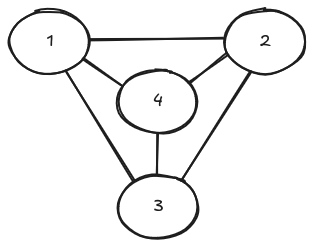
\includegraphics[scale=0.5]{6.png}
\columnbreak
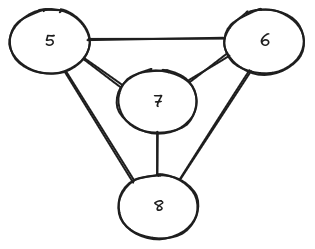
\includegraphics[scale=0.5]{7.png}
\end{multicols}
\end{center}

\begin{center}
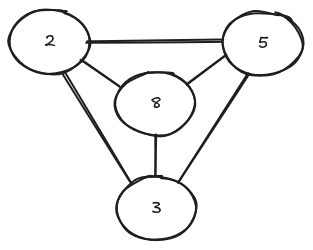
\includegraphics[scale=0.5]{9.png}
\end{center}

\vspace{5mm}

\begin{minted}{console}
[...]$ ./build/cmd/gmp/cpp/ucg-add 1.txt 2.txt 3.txt
1: 2 3 4 
2: 1 3 4 5 8 
3: 1 2 4 5 8 
4: 1 2 3 
5: 2 3 6 7 8 
6: 5 7 8 
7: 5 6 8 
8: 2 3 5 6 7
\end{minted}

\vspace{5mm}

\begin{center}
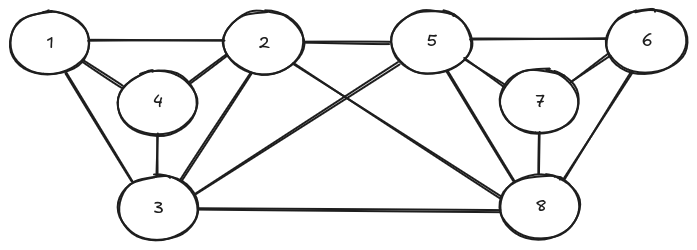
\includegraphics[scale=0.5]{8.png}
\end{center}

\end{document}

